% Shared standalone design for the editable figure reconstructions.
\documentclass[tikz,border=5pt,10pt]{standalone}
\usepackage[T1]{fontenc}
\usepackage[utf8]{inputenc}
\usepackage{newpxtext,newpxmath}
\usepackage[scaled=.94]{sourcesanspro}
\usepackage{pgfplots}
\pgfplotsset{compat=1.18}
\usetikzlibrary{arrows.meta,calc,positioning,decorations.pathreplacing,
  decorations.markings,patterns,matrix,shapes.geometric,fit,backgrounds,
  intersections,angles,quotes}
\definecolor{ink}{HTML}{203746}
\definecolor{accent}{HTML}{146C78}
\definecolor{muted}{HTML}{667780}
\definecolor{signalred}{HTML}{B94B44}
\color{ink}
\tikzset{>=Latex,line width=.8pt,
  every node/.style={font=\small},
  axis/.style={->,draw=muted,line width=.5pt},
  guide/.style={draw=muted,dashed,line width=.45pt},
  curve/.style={draw=accent,line width=1pt},
  marker/.style={circle,fill=accent,inner sep=1.5pt},
  labelbox/.style={fill=white,inner sep=2pt}}

\begin{document}
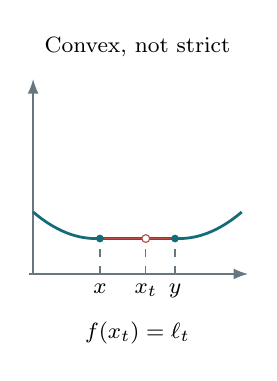
\begin{tikzpicture}[x=.53cm,y=.75cm,every node/.style={font=\footnotesize}]
\draw[axis] (-2.6,0)--(2.65,0);\draw[axis] (-2.5,0)--(-2.5,3.3);
\draw[curve,domain=-2.5:2.5,samples=200] plot (\x,{.2*max(abs(\x)-1,0)^2+.6});
\draw[signalred] (-0.9,0.6)--(0.9,0.6);\draw[signalred,dashed] (0.2,0.6)--(0.2,0.6);
\draw[guide] (-0.9,0)--(-0.9,0.6);\fill[accent] (-0.9,0.6) circle(1.4pt);\node[below] at (-0.9,0) {$x$};
\draw[guide] (0.2,0)--(0.2,0.6);\fill[accent] (0.2,0.6) circle(1.4pt);\node[below] at (0.2,0) {$x_t$};
\draw[guide] (0.9,0)--(0.9,0.6);\fill[accent] (0.9,0.6) circle(1.4pt);\node[below] at (0.9,0) {$y$};
\draw[signalred,fill=white] (0.2,0.6) circle(1.4pt);
\node at (0,3.85) {Convex, not strict};\node at (0,-1) {$f(x_t)=\ell_t$};
\end{tikzpicture}
\end{document}
